\documentclass[aspectratio=169]{beamer}

% ===== Plain lecture-slide style: blue frame titles, blue triangle bullets =====
\usetheme{default}

\setbeamertemplate{navigation symbols}{}
\setbeamertemplate{frametitle}[default][left]
\setbeamertemplate{itemize items}[triangle]

% Beamer blue used in the lecture slides
\definecolor{lmublue}{RGB}{47,47,140}
\setbeamercolor{frametitle}{fg=lmublue,bg=}
\setbeamercolor{title}{fg=lmublue}
\setbeamercolor{subtitle}{fg=black}
\setbeamercolor{structure}{fg=lmublue}   % bullets and block titles
\setbeamerfont{frametitle}{series=\bfseries,size=\large}

% Bottom info bar: blue background, white text (as in the lecture slides)
\setbeamercolor{author in head/foot}{fg=white,bg=lmublue}
\setbeamercolor{title in head/foot}{fg=white,bg=lmublue}
\setbeamercolor{date in head/foot}{fg=white,bg=lmublue}
\setbeamertemplate{footline}{%
  \hbox{%
    \begin{beamercolorbox}[wd=.34\paperwidth,ht=2.5ex,dp=1ex,leftskip=1em]{author in head/foot}%
      \usebeamerfont{author in head/foot}\insertshortauthor%
    \end{beamercolorbox}%
    \begin{beamercolorbox}[wd=.40\paperwidth,ht=2.5ex,dp=1ex,center]{title in head/foot}%
      \usebeamerfont{title in head/foot}\insertshorttitle%
    \end{beamercolorbox}%
    \begin{beamercolorbox}[wd=.26\paperwidth,ht=2.5ex,dp=1ex,rightskip=1em]{date in head/foot}%
      \usebeamerfont{date in head/foot}\hfill\insertframenumber\,/\,\inserttotalframenumber%
    \end{beamercolorbox}%
  }%
}

\usepackage[utf8]{inputenc}
\usepackage[T1]{fontenc}
\usepackage{amsmath,amssymb}
\usepackage{booktabs}
\usepackage{graphicx}
\usepackage{multirow}
\usepackage{subcaption}

\title[Lag-Order Uncertainty in Set-Identified SVARs]{Lag-Order Uncertainty in Set-Identified SVARs}
\subtitle{A comparative presentation of two Monte Carlo studies}
\author[Ak\i n Ayd\i n \& Ferdinand Loser]{Ak\i n Ayd\i n \and Ferdinand Loser}
\institute{Ludwig-Maximilian University of Munich}
\date{\today}

\begin{document}

\begin{frame}
  \titlepage
\end{frame}

\begin{frame}{Agenda}
  \tableofcontents
\end{frame}


\begin{frame}{Introduction}
  \begin{itemize}
    \item Inspiration from Ivanov and Kilian (2005) who compare the performance of different lag-order selection criteria in a Monte Carlo study in how well they can recover the true IRF of a VAR model.
    \item Since then VAR estimation has changed a lot, we aim to update their analysis to a more current framework:
  \end{itemize}
  \begin{table}
        \begin{tabular}{@{} l p{5cm} p{5cm} @{}}
            \toprule
            \textbf{Feature} & \textbf{Ivanov and Kilian (2005)} & \textbf{Our Approach} \\
            \midrule
            IRF & Point-Identified (Cholesky Decomposition) & Set-Identified (Sign Restrictions) \\ 
            \addlinespace
            Model Selection & Information Criteria & Information Criteria vs. BVAR and BMA \\
            \addlinespace
            Data & Macroeconomic Studies from the 1990s/early 2000s (both monthly and quarterly) & Kilian and Murphy (2012) (monthly)\\
            \bottomrule
        \end{tabular}
    \end{table}
\end{frame}

\begin{frame}{Simulation Design}
  \begin{itemize}
    \item Using VAR specification with true IRF specific $\tilde{B}$ to median target IRF from intitial estimation on real data from Kilian and Murphy (2012).
    \item Estimation for lag orders $p_0 \in \{4,10\}$, and sample sizes $T \in \{240, 360, 480, 600\}$
    \item 500 Monte Carlo iterations $R$ for each combination of $p_0$ and $T$, 1000 admissible IRFs selected for each model in each iteration. \\
    (Computational limits even with parallel processing and translation into machine code with \texttt{numba} and \texttt{joblib} packages in \texttt{python})
    \item Metric for performance comparison: Geometric mean of squared errors of median IRF of model $j$ relative to the median IRF of a model correctly specified with $p_0$:
  \end{itemize}
\begin{equation}
    MSE^{relative}_j = \exp\left( \frac{1}{n} \sum_{i=1}^{R} \ln(\frac{SE_{ji}}{SE_{p_0i}}) \right)
\end{equation}
\end{frame}

\section{Results}

\begin{frame}{IC Lag Selection}
  \begin{table}[htbp]
\centering
\caption{Average Evaluated Lag Order ($\hat{p}$) selected by Information Criteria.}
\label{tab:ic_lag_orders}
\begin{tabular}{llccc}
\toprule
 & Estimator & AIC & BIC & HQC \\
$p_0$ & $T$ &  &  &  \\
\midrule
\multirow[t]{2}{*}{4} & 240 & 2.99 & 1.95 & 2.06 \\
 & 600 & 3.80 & 2.02 & 2.66 \\
\multirow[t]{2}{*}{10} & 240 & 6.54 & 1.96 & 2.07 \\
 & 600 & 9.16 & 2.02 & 4.03 \\
\bottomrule
\end{tabular}
\end{table}

\end{frame}

\begin{frame}{IC Performance Comparison}
  \begin{table}[htbp]
\centering
\caption{Relative Mean Squared Error: Information Criteria Baselines.}
\label{tab:ic_mse_baselines}
\noindent\sbox0{\begin{tabular}{llccc}
\toprule
 &  & AIC & BIC & HQC \\
$p_0$ & $T$ &  &  &  \\
\midrule
\multirow[t]{4}{*}{4} & 240 & \bfseries 1.083 & 1.108 & 1.129 \\
 & 360 & \bfseries 1.117 & 1.274 & 1.296 \\
 & 480 & \bfseries 0.986 & 1.133 & 1.124 \\
 & 600 & \bfseries 0.989 & 1.145 & 1.118 \\
\multirow[t]{4}{*}{10} & 240 & 1.033 & \bfseries 1.018 & 1.021 \\
 & 360 & \bfseries 0.811 & 0.904 & 0.878 \\
 & 480 & \bfseries 0.989 & 1.190 & 1.185 \\
 & 600 & \bfseries 1.036 & 1.260 & 1.259 \\
\bottomrule
\end{tabular}}
\noindent\usebox0\par
                \vspace{1ex}
                \noindent\begin{minipage}{\wd0}
                \raggedright\footnotesize\textit{Note:} Bold values indicate the lowest Relative Mean Squared Error across the respective scenario.
                \end{minipage}
\end{table}

\end{frame}

\begin{frame}{BVAR vs. IC Performance Comparison}
  \begin{table}[htbp]
\centering
\caption{Relative Mean Squared Error of Bayesian Shrinkage Specifications vs.~AIC Baseline.}
\label{tab:bvar_vs_aic}
\begin{tabular}{llccccc}
\toprule
 &  & \begin{tabular}{@{}c@{}}BVAR \\ ($\lambda_1=0.20$)\end{tabular} & \begin{tabular}{@{}c@{}}BVAR \\ ($\lambda_1=0.40$)\end{tabular} & \begin{tabular}{@{}c@{}}BVAR \\ ($\lambda_1=0.60$)\end{tabular} & \begin{tabular}{@{}c@{}}BVAR \\ ($\lambda_1=0.80$)\end{tabular} & \begin{tabular}{@{}c@{}}BVAR \\ (MDD $\lambda_1$)\end{tabular} \\
$T$ & $p_0$ &  &  &  &  &  \\
\midrule
\multirow[t]{2}{*}{240} & 4 & 0.981 & \bfseries 0.974 & 0.994 & 1.057 & 0.981 \\
 & 10 & 0.866 & 0.858 & \bfseries 0.840 & 0.917 & 0.866 \\
\multirow[t]{2}{*}{360} & 4 & 0.922 & 1.045 & \bfseries 0.890 & 1.022 & 0.922 \\
 & 10 & 1.105 & 1.110 & \bfseries 1.055 & 1.116 & 1.124 \\
\multirow[t]{2}{*}{480} & 4 & 1.153 & 1.125 & \bfseries 1.108 & 1.116 & 1.153 \\
 & 10 & \bfseries 0.863 & 0.931 & 0.886 & 0.955 & 0.876 \\
\multirow[t]{2}{*}{600} & 4 & 1.145 & \bfseries 0.994 & 1.115 & 1.122 & 1.145 \\
 & 10 & \bfseries 0.782 & 0.865 & 0.819 & 0.791 & 0.796 \\
\bottomrule
\end{tabular}
\end{table}

\end{frame}


\begin{frame}{BVAR Performance Depending on $\lambda_1$}
\begin{figure} % The [p] tells LaTeX to put this on its own dedicated page
    \centering
    
    % Top Left: Figure 5
    \begin{subfigure}[b]{0.48\textwidth}
        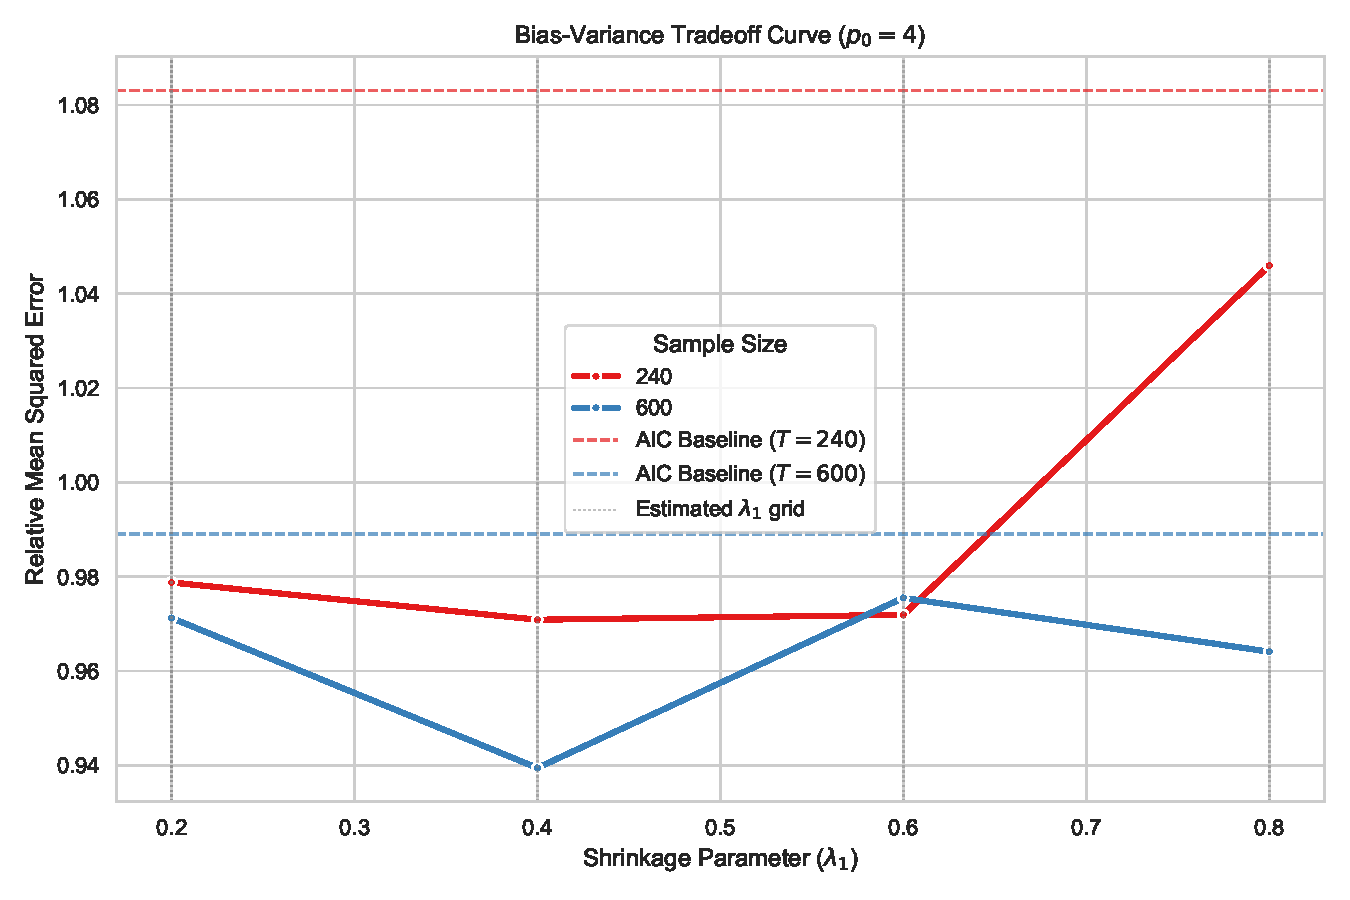
\includegraphics[width=\textwidth]{Figures/Fig1_Tradeoff_Curve.pdf}
        \caption{$p_0=4$}
    \label{fig:tradeoff_p4}
    \end{subfigure}
    \hfill % Adds horizontal space between the two columns
    % Top Right: Figure 6
    \begin{subfigure}[b]{0.48\textwidth}
        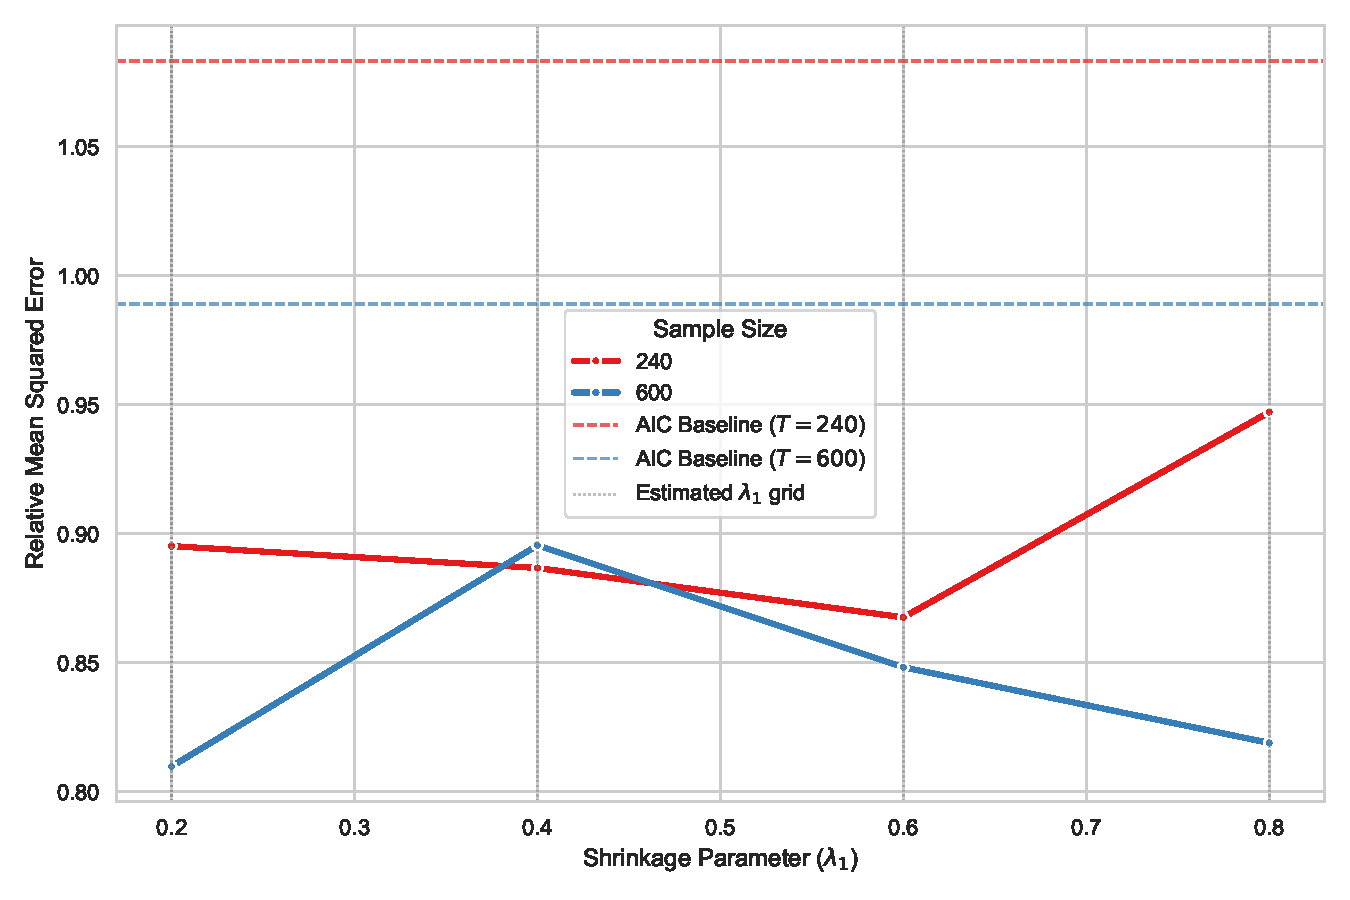
\includegraphics[width=\textwidth]{Figures/Fig1_Tradeoff_Curve_p10.pdf}
        \caption{$p_0=10$}
    \label{fig:tradeoff_p10}
    \end{subfigure}
  
    \caption{Comparison of BVAR's performance across different $\lambda_1$-values in comparison to AIC.}
    \label{fig:tradeoff}
\end{figure}
\end{frame}

\begin{frame}{MDD Selection of $\lambda_1$}
  \begin{figure}[htbp]
    \centering
    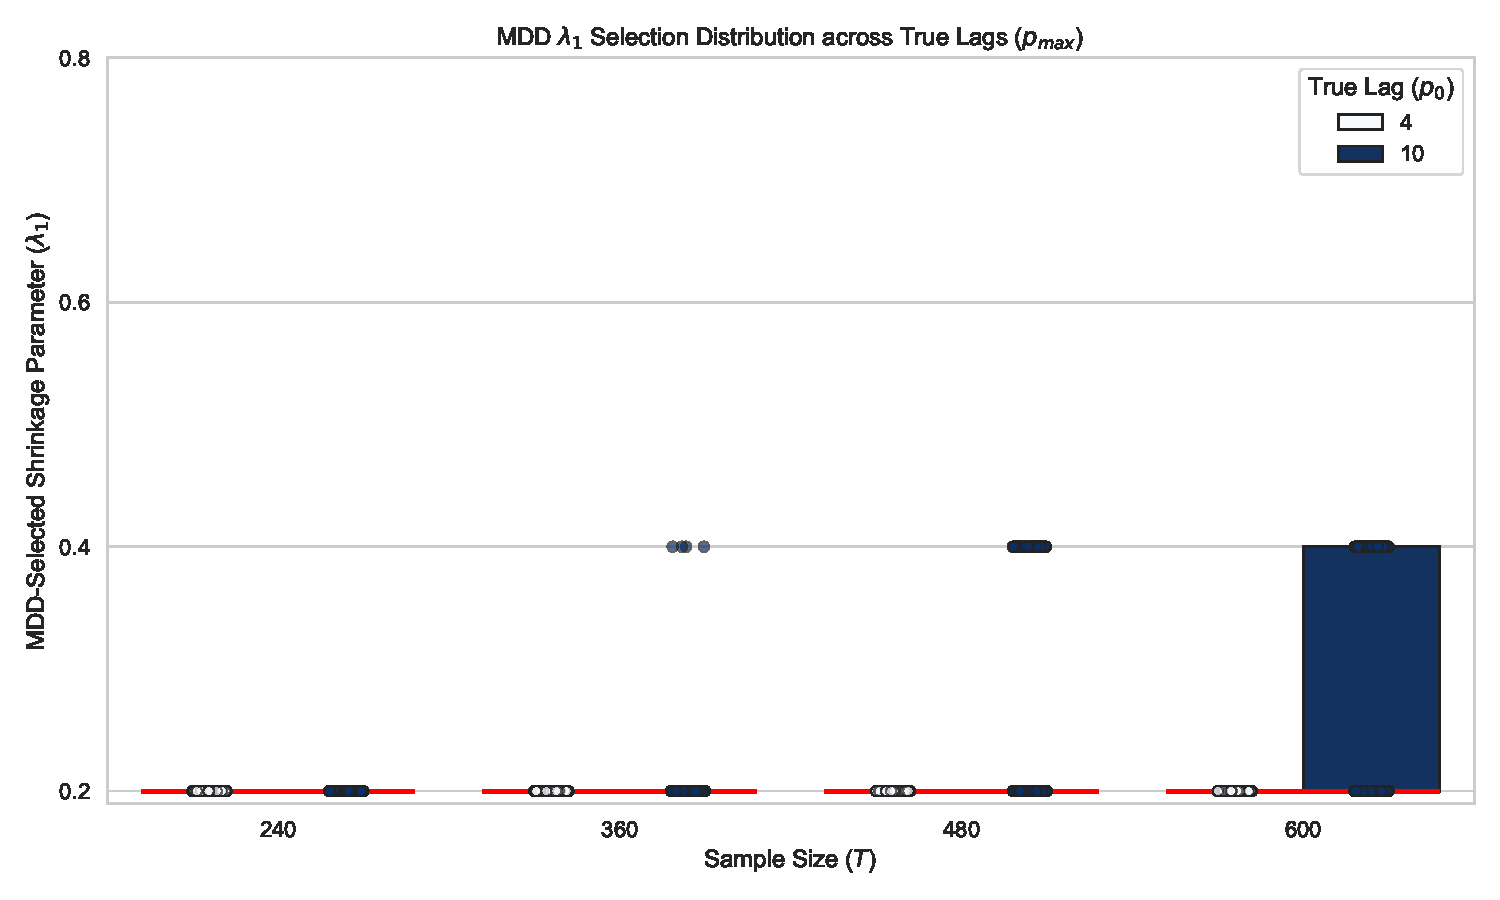
\includegraphics[width=0.65\textwidth]{Figures/Fig2_Asymptotic_Relaxation.pdf}
    \caption{The MDD selected hyperparameter $\lambda_1$ for different sample sizes (both $p_0=4$ and $p_0=10$).}
    {\raggedright \footnotesize \textbf{Note:} Circles represent optimal $\lambda_1$-values in individual iterations, bars represent the interquartile range, red lines indicate the median. \par}
\label{fig:asymptotic_relaxation}
\end{figure}
\end{frame}

\begin{frame}{BMA vs. IC Performance Comparison}
  \input{Tables/Table8_BMA_vs_AIC.tex}
\end{frame}
\begin{frame}{BMA Weighting (OLS BMA - BIC)}
\begin{figure} % The [p] tells LaTeX to put this on its own dedicated page
    \centering
    
    % Top Left: Figure 5
    \begin{subfigure}[b]{0.48\textwidth}
        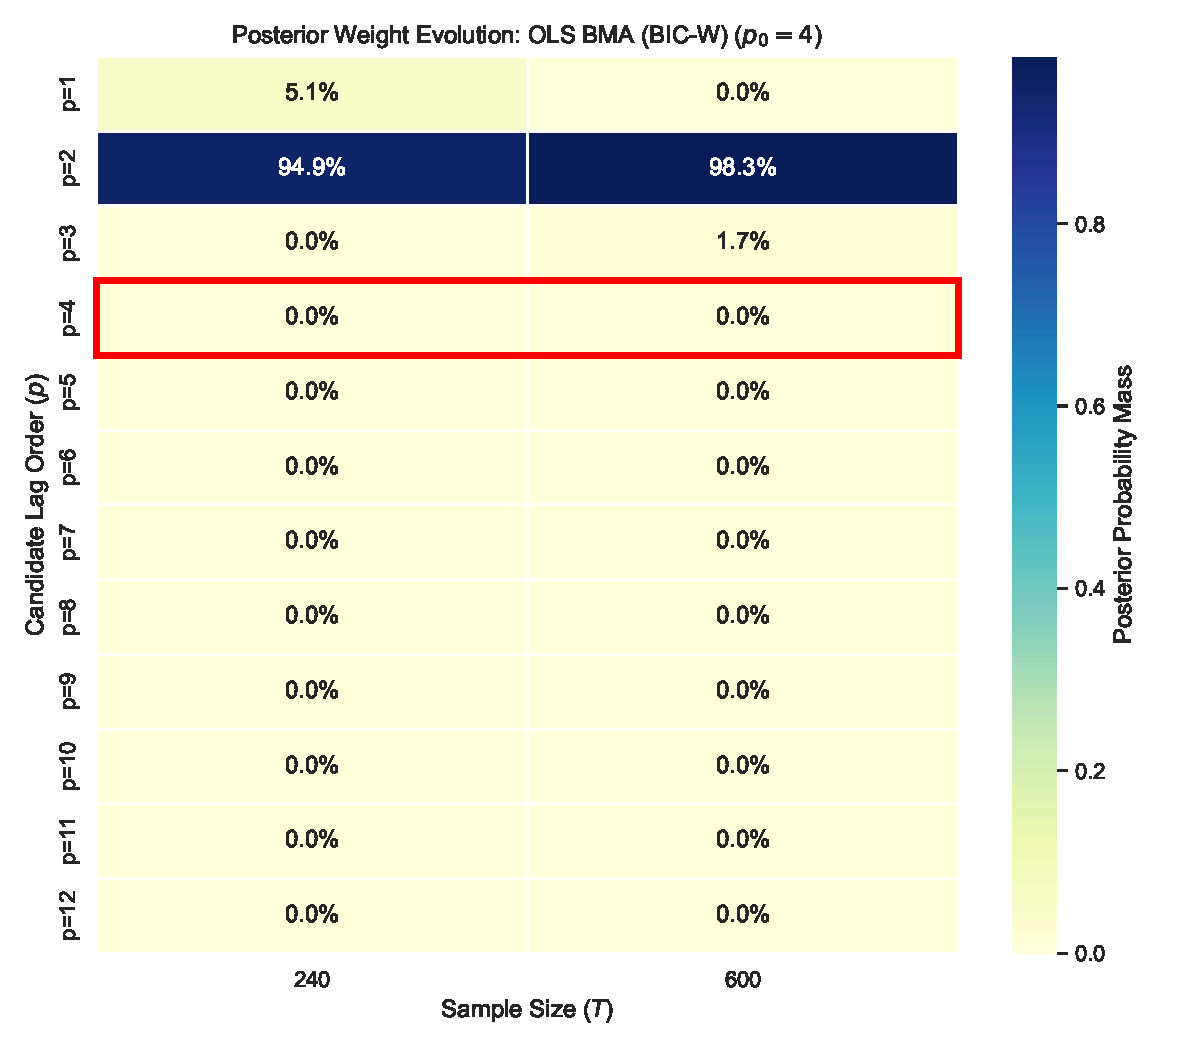
\includegraphics[width=\textwidth]{Figures/Fig5a_BMA_Heatmap_OLS.pdf}
        \caption{OLS BMA (BIC-weighted)}
        \label{fig:heat_ols}
    \end{subfigure}
    \hfill % Adds horizontal space between the two columns
    % Top Right: Figure 6
    \begin{subfigure}[b]{0.48\textwidth}
        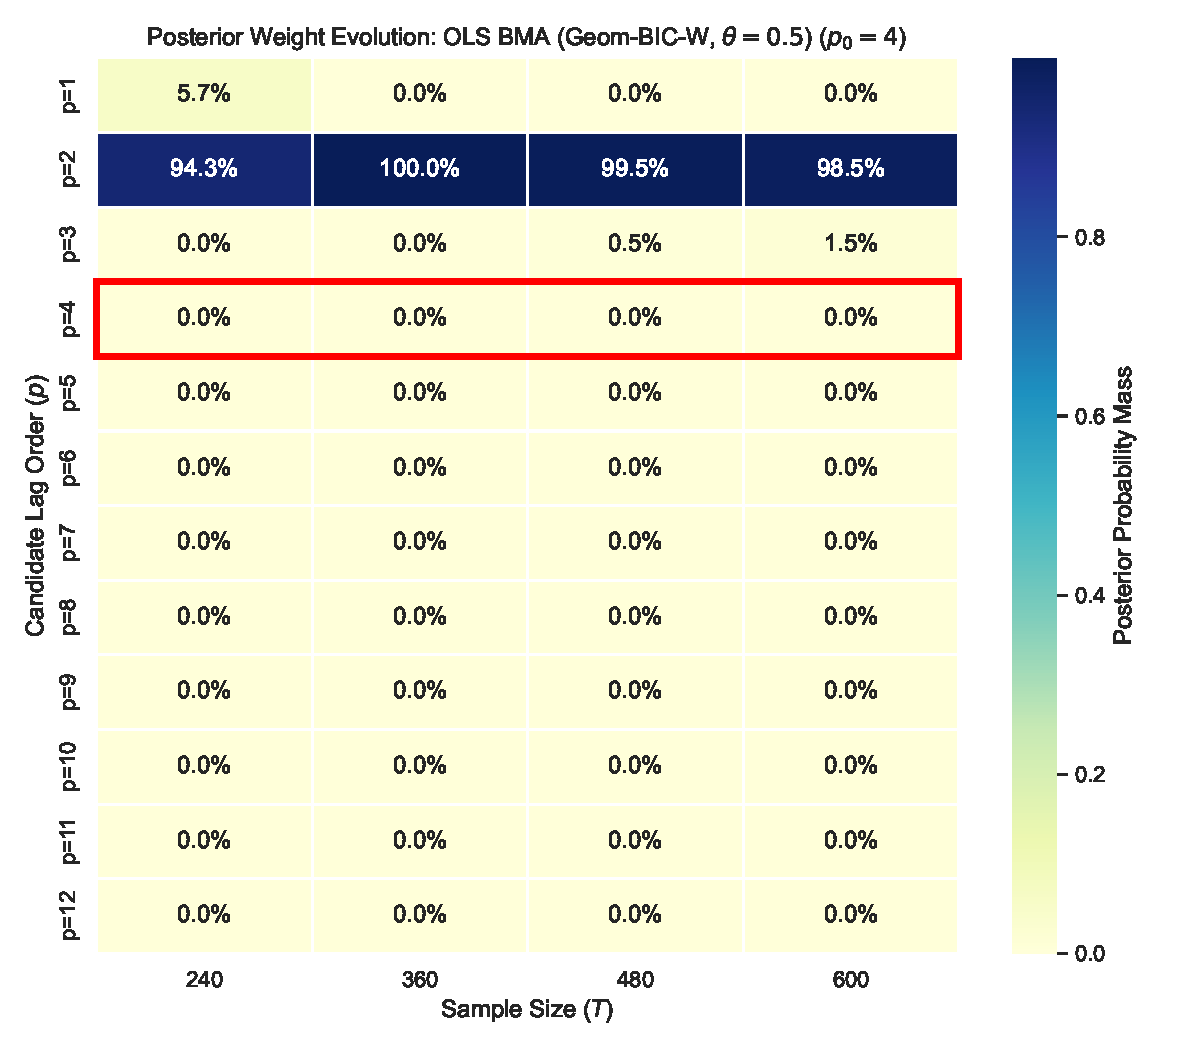
\includegraphics[width=\textwidth]{Figures/Fig5b_BMA_Heatmap_OLS_Geom.pdf}
        \caption{OLS BMA (Geom. BIC-weighted, $\theta=0.5$)}
        \label{fig:heat_ols_geom}
    \end{subfigure}
\end{figure}  
\end{frame}

\begin{frame}{BMA Weighting (OLS BMA - AIC)}
\begin{figure}
    \centering
    % Bottom Left: Figure 7
    \begin{subfigure}[b]{0.48\textwidth}
        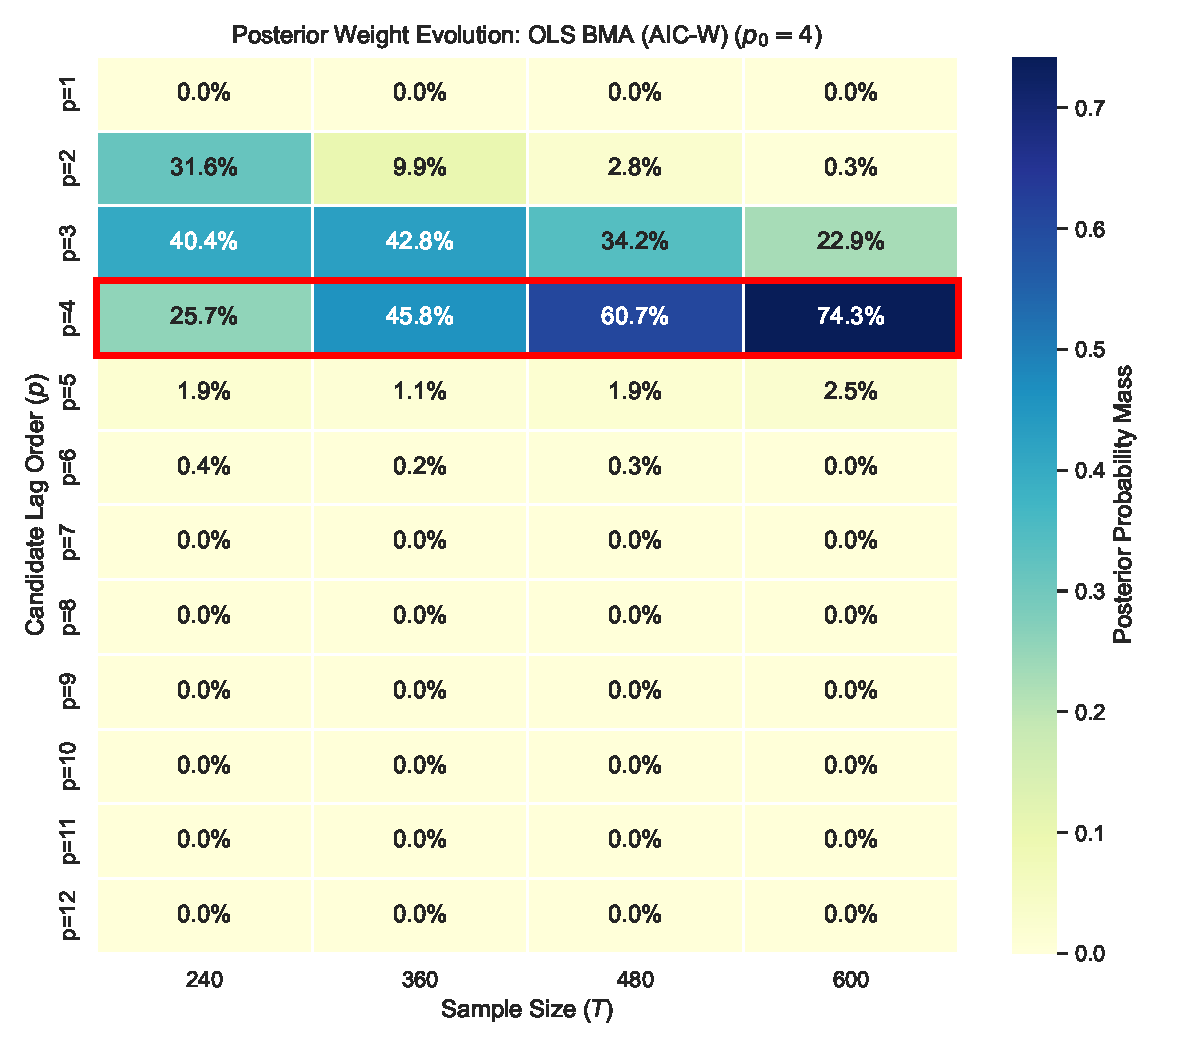
\includegraphics[width=\textwidth]{Figures/Fig5c_BMA_Heatmap_OLS_AIC.pdf}
        \caption{OLS BMA (AIC-weighted)}
        \label{fig:heat_aic}
    \end{subfigure}
    \hfill
    % Bottom Right: Figure 8
    \begin{subfigure}[b]{0.48\textwidth}
        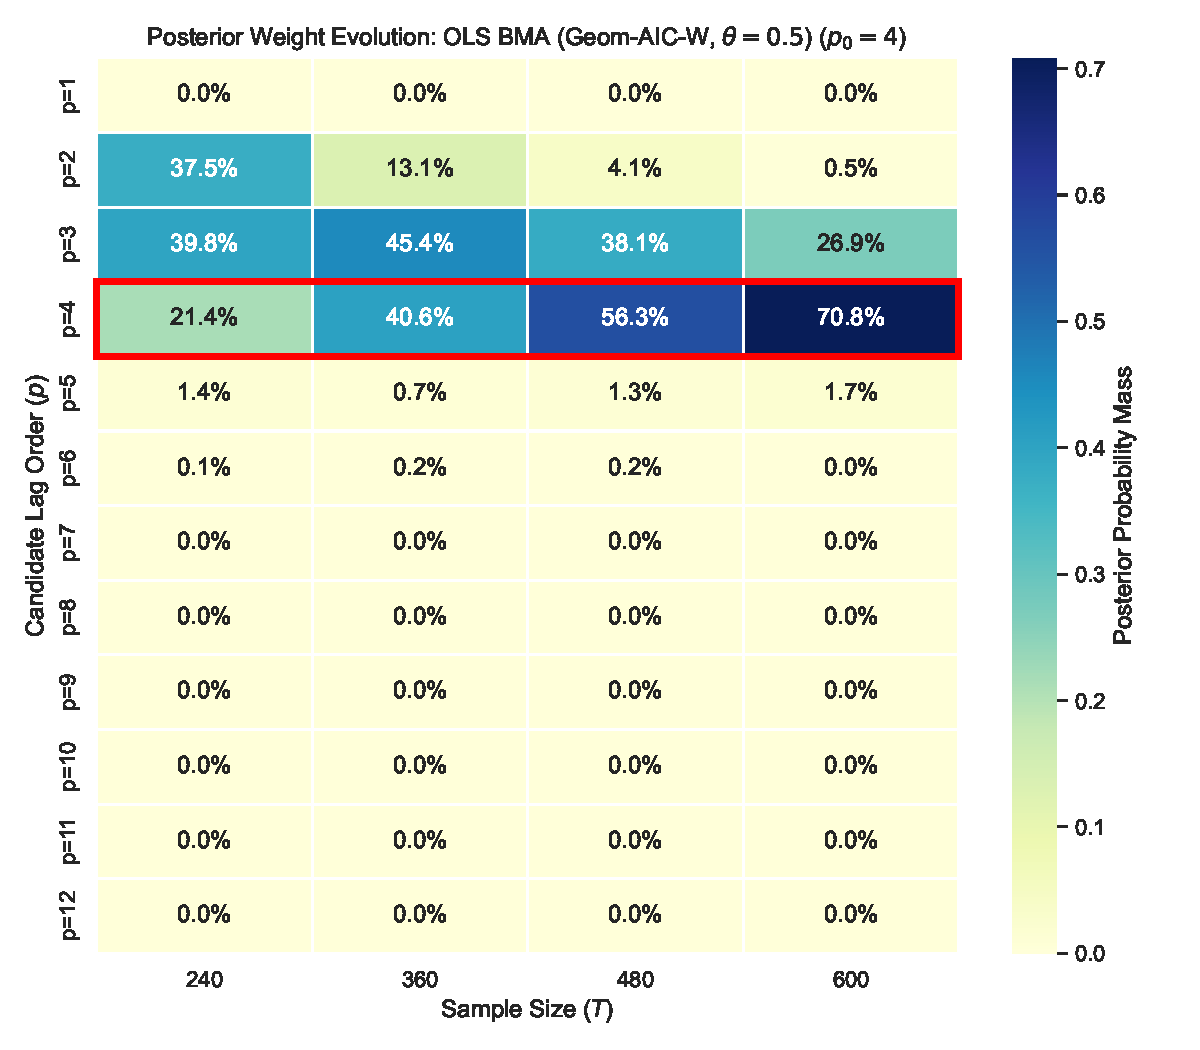
\includegraphics[width=\textwidth]{Figures/Fig5d_BMA_Heatmap_OLS_Geom_AIC.pdf}
        \caption{OLS BMA (Geom. AIC-weighted, $\theta=0.5$)}
        \label{fig:heat_aic_geom}
    \end{subfigure}
    
    \caption{Posterior Weight Evolution across the four OLS BMA architectures ($p_0=4$).}
    \label{fig:bma_heatmaps_grid}
\end{figure}  
\end{frame}

\begin{frame}{BMA Weighting (Aggreagated for both Grid Approaches)}
\begin{figure} % The [p] tells LaTeX to put this on its own dedicated page
    \centering
    
    % Top Left: Figure 5
    \begin{subfigure}[b]{0.48\textwidth}
        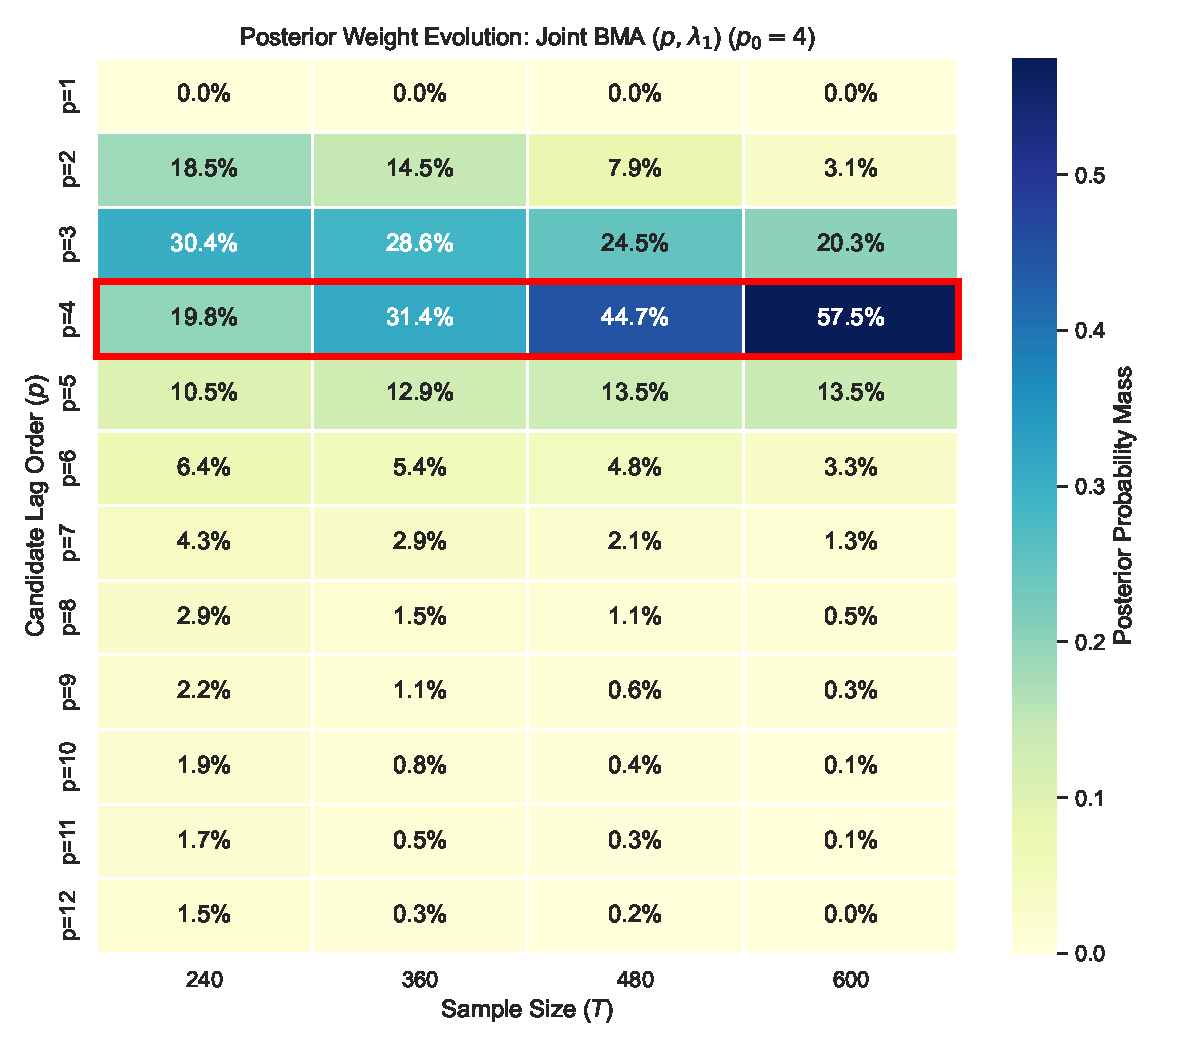
\includegraphics[width=\textwidth]{Figures/Fig5e_BMA_Heatmap_Joint.pdf}
        \caption{Joint Grid BMA}
        \label{fig:heat_joint}
    \end{subfigure}
    \hfill % Adds horizontal space between the two columns
    % Top Right: Figure 6
    \begin{subfigure}[b]{0.48\textwidth}
        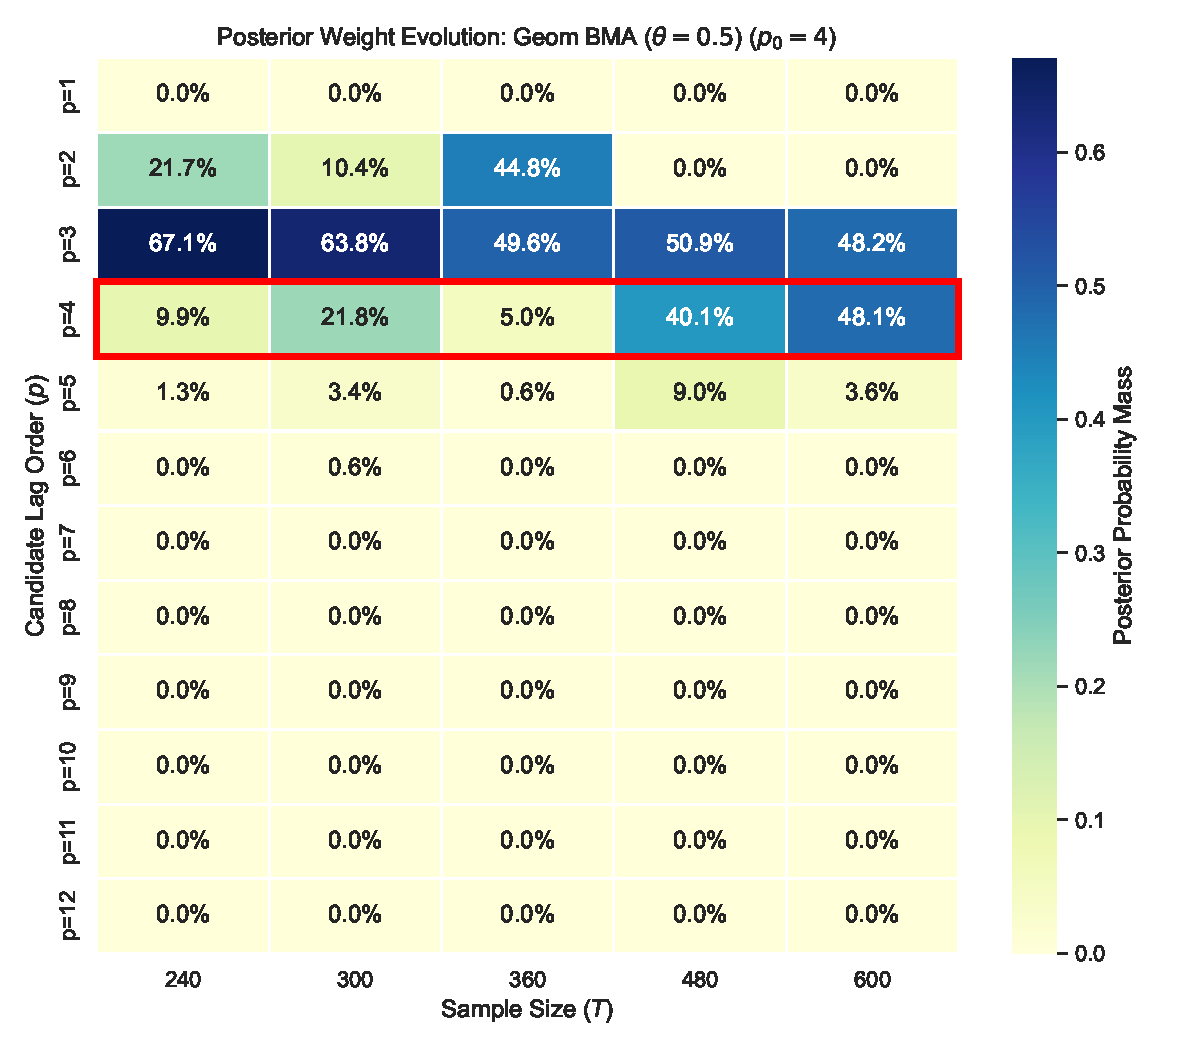
\includegraphics[width=\textwidth]{Figures/Fig5f_BMA_Heatmap_Geom.pdf}
        \caption{Geometric Grid BMA}
        \label{fig:heat_geom}
    \end{subfigure}
  
    \caption{Posterior Weight Evolution for the two BVAR-based BMAs ($p_0=4$).}
    \label{fig:bma_heatmaps_grid_bvar}
\end{figure} 
\end{frame}

\begin{frame}{Average shrinkage changes with $p$}
\begin{figure}[htbp]
    \centering
    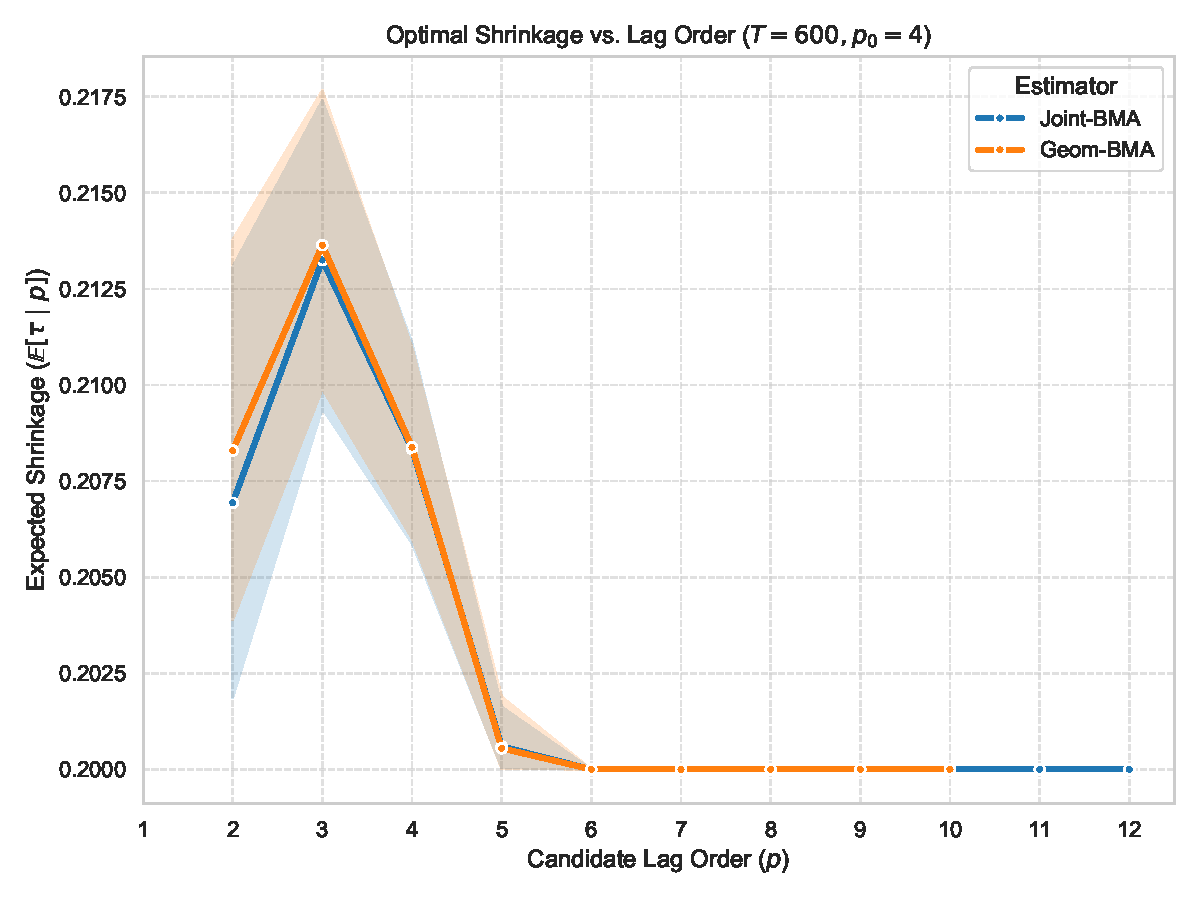
\includegraphics[width=0.65\textwidth]{Figures/Fig9_Tau_Comparison_T600_p04.pdf}
    \caption{The expected weight of $\lambda_1$ given $p$ changes with $p$ ($p_0=4$).}
    \label{fig:tau_to_p}
\end{figure}
\end{frame}

\begin{frame}{Performance of BMA vs Hard Selection at Different Sample Sizes}
\begin{figure}[p] % The [p] tells LaTeX to put this on its own dedicated page
    \centering
    
    \begin{subfigure}[b]{0.48\textwidth}
        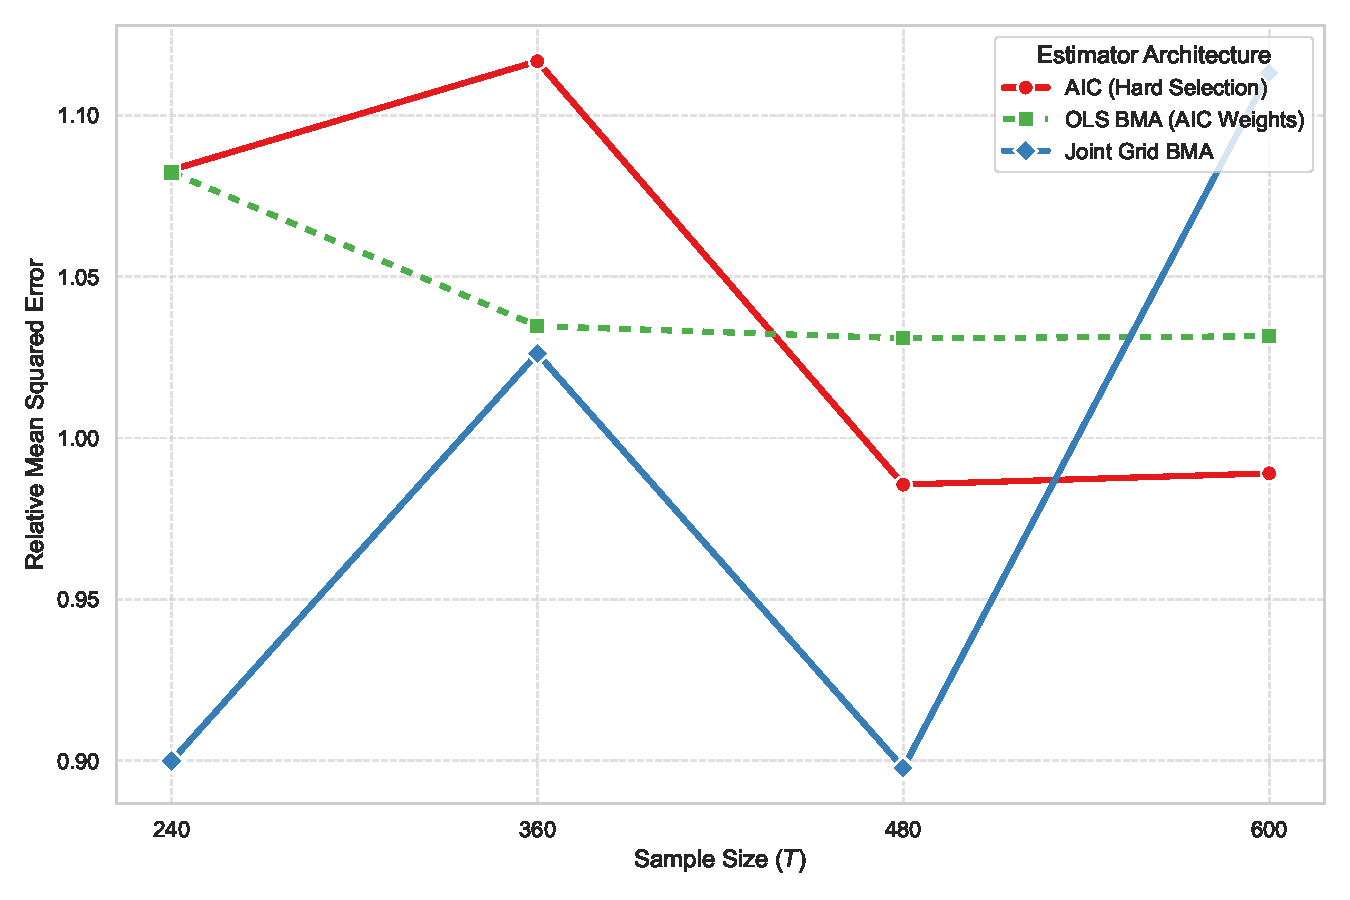
\includegraphics[width=\textwidth]{Figures/Fig1b_Asymptotic_Convergence_p4.pdf}
        \caption{$p_0=4$}
        \label{fig:convergence4}
    \end{subfigure}
    \hfill % Adds horizontal space between the two columns
    \begin{subfigure}[b]{0.48\textwidth}
        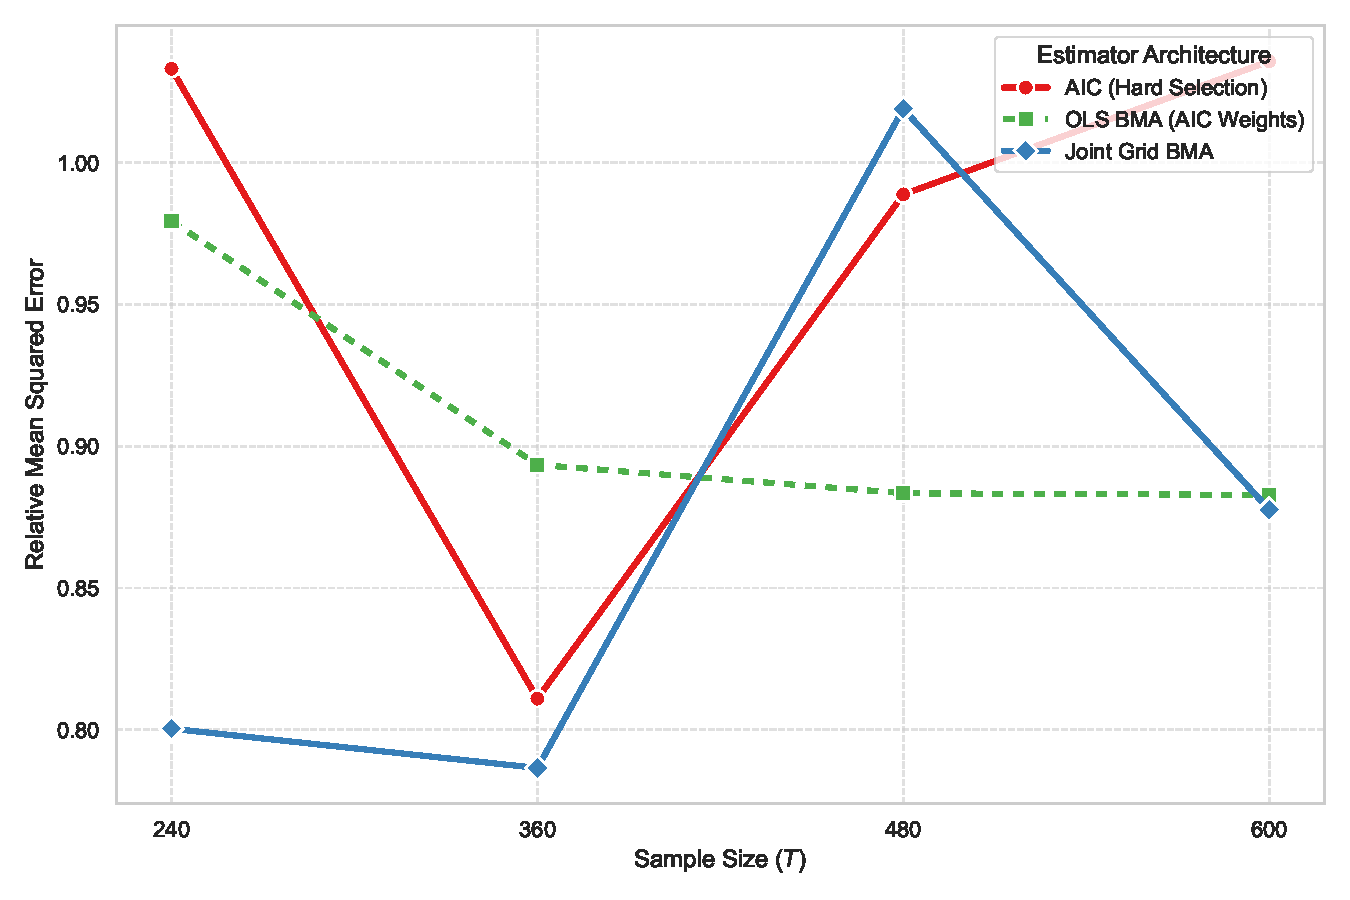
\includegraphics[width=\textwidth]{Figures/Fig1c_Asymptotic_Convergence_p10.pdf}
        \caption{$p_0=10$}
        \label{fig:convergence10}
    \end{subfigure}
  
    \caption{Performance of BMA vs Hard Selection at different sample sizes $T$.}
    \label{fig:convergence}
\end{figure}
\end{frame}



\end{document}